\section{实验结果与分析}

本章节将介绍本次实验的结果与分析,包括实验结果的展示,消融实验的结果,实验结果的分析等。

\subsection{实验结果}

图\ref{fig:results}展示了实验结果,包括特征点的检测与匹配。

% 5张子图网格排列,images/log.png, images/results/vis_circles.jpg, images/results/vis_lines.jpg, images/results/eval.jpg, images/acc.png
% A B
% C D
% E
% use \subfloat
\begin{figure}[H]
    \centering
    \subfloat [中间日志信息] {
        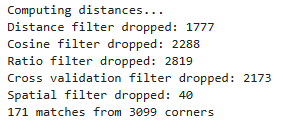
\includegraphics[width=0.5\textwidth]{images/log.png}
    }
    \subfloat [特征点检测结果] {
        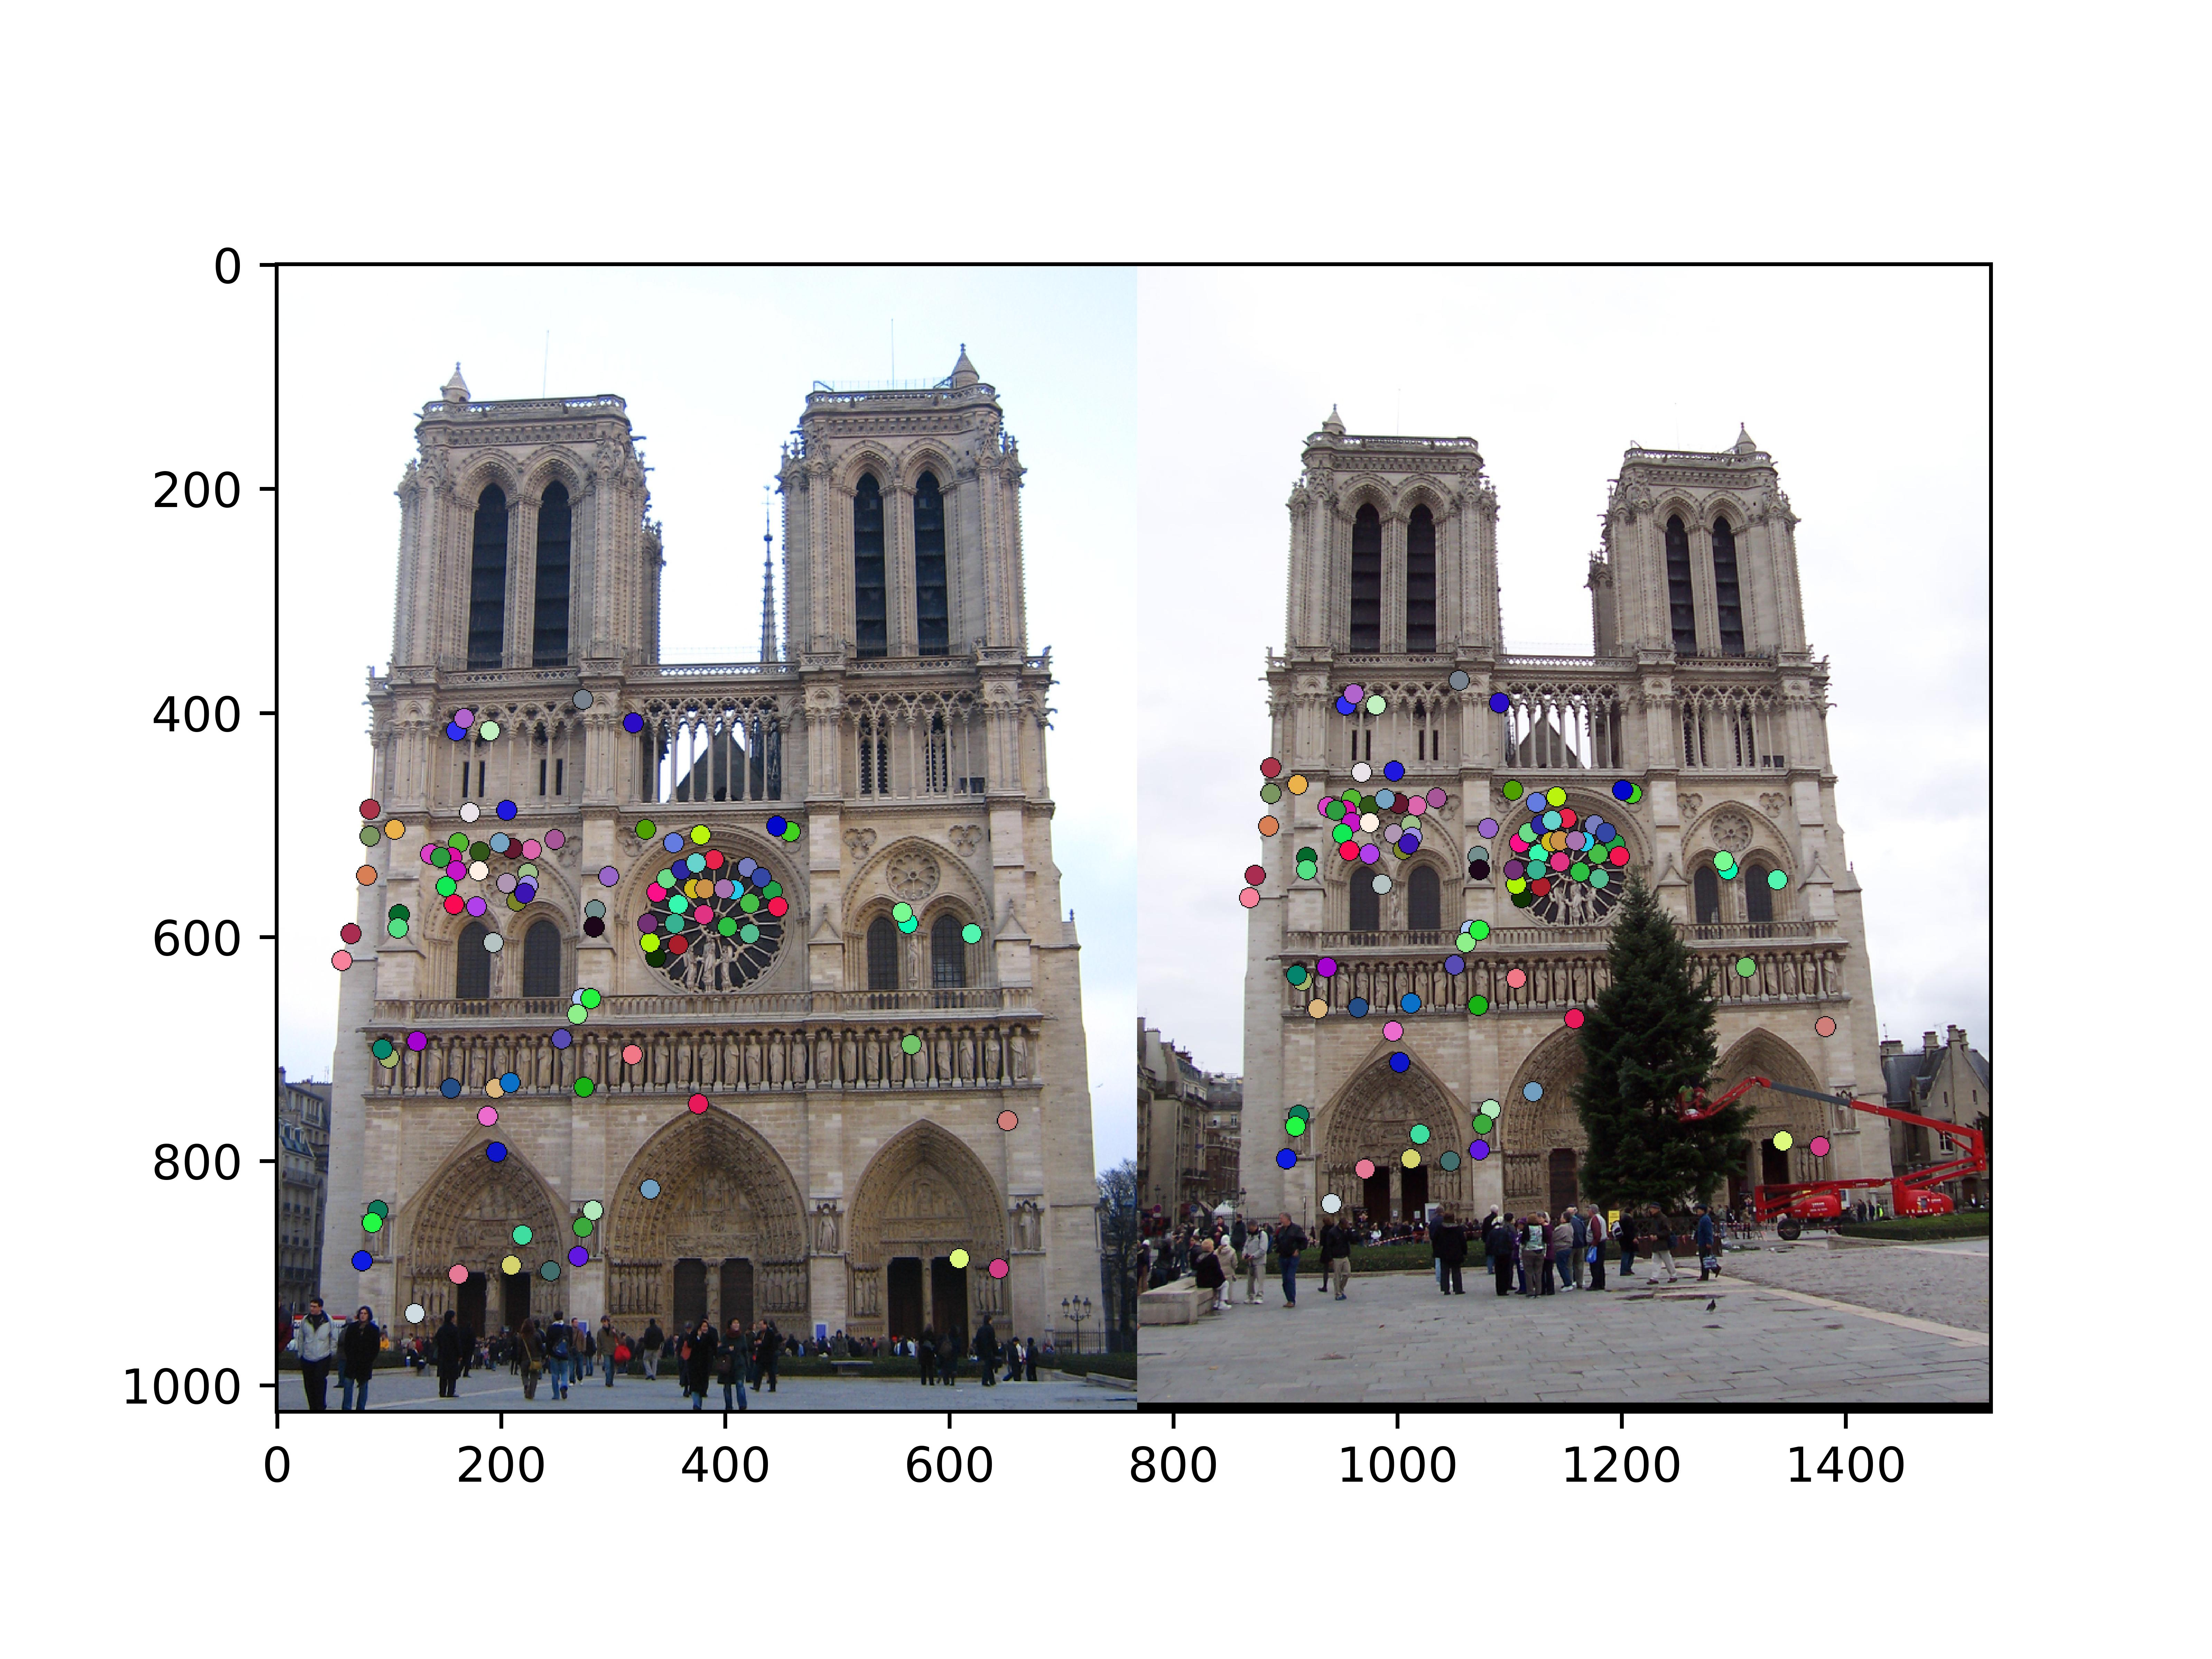
\includegraphics[width=0.5\textwidth]{images/results/vis_circles.jpg}
    }
    \\
    \subfloat [特征点匹配结果] {
        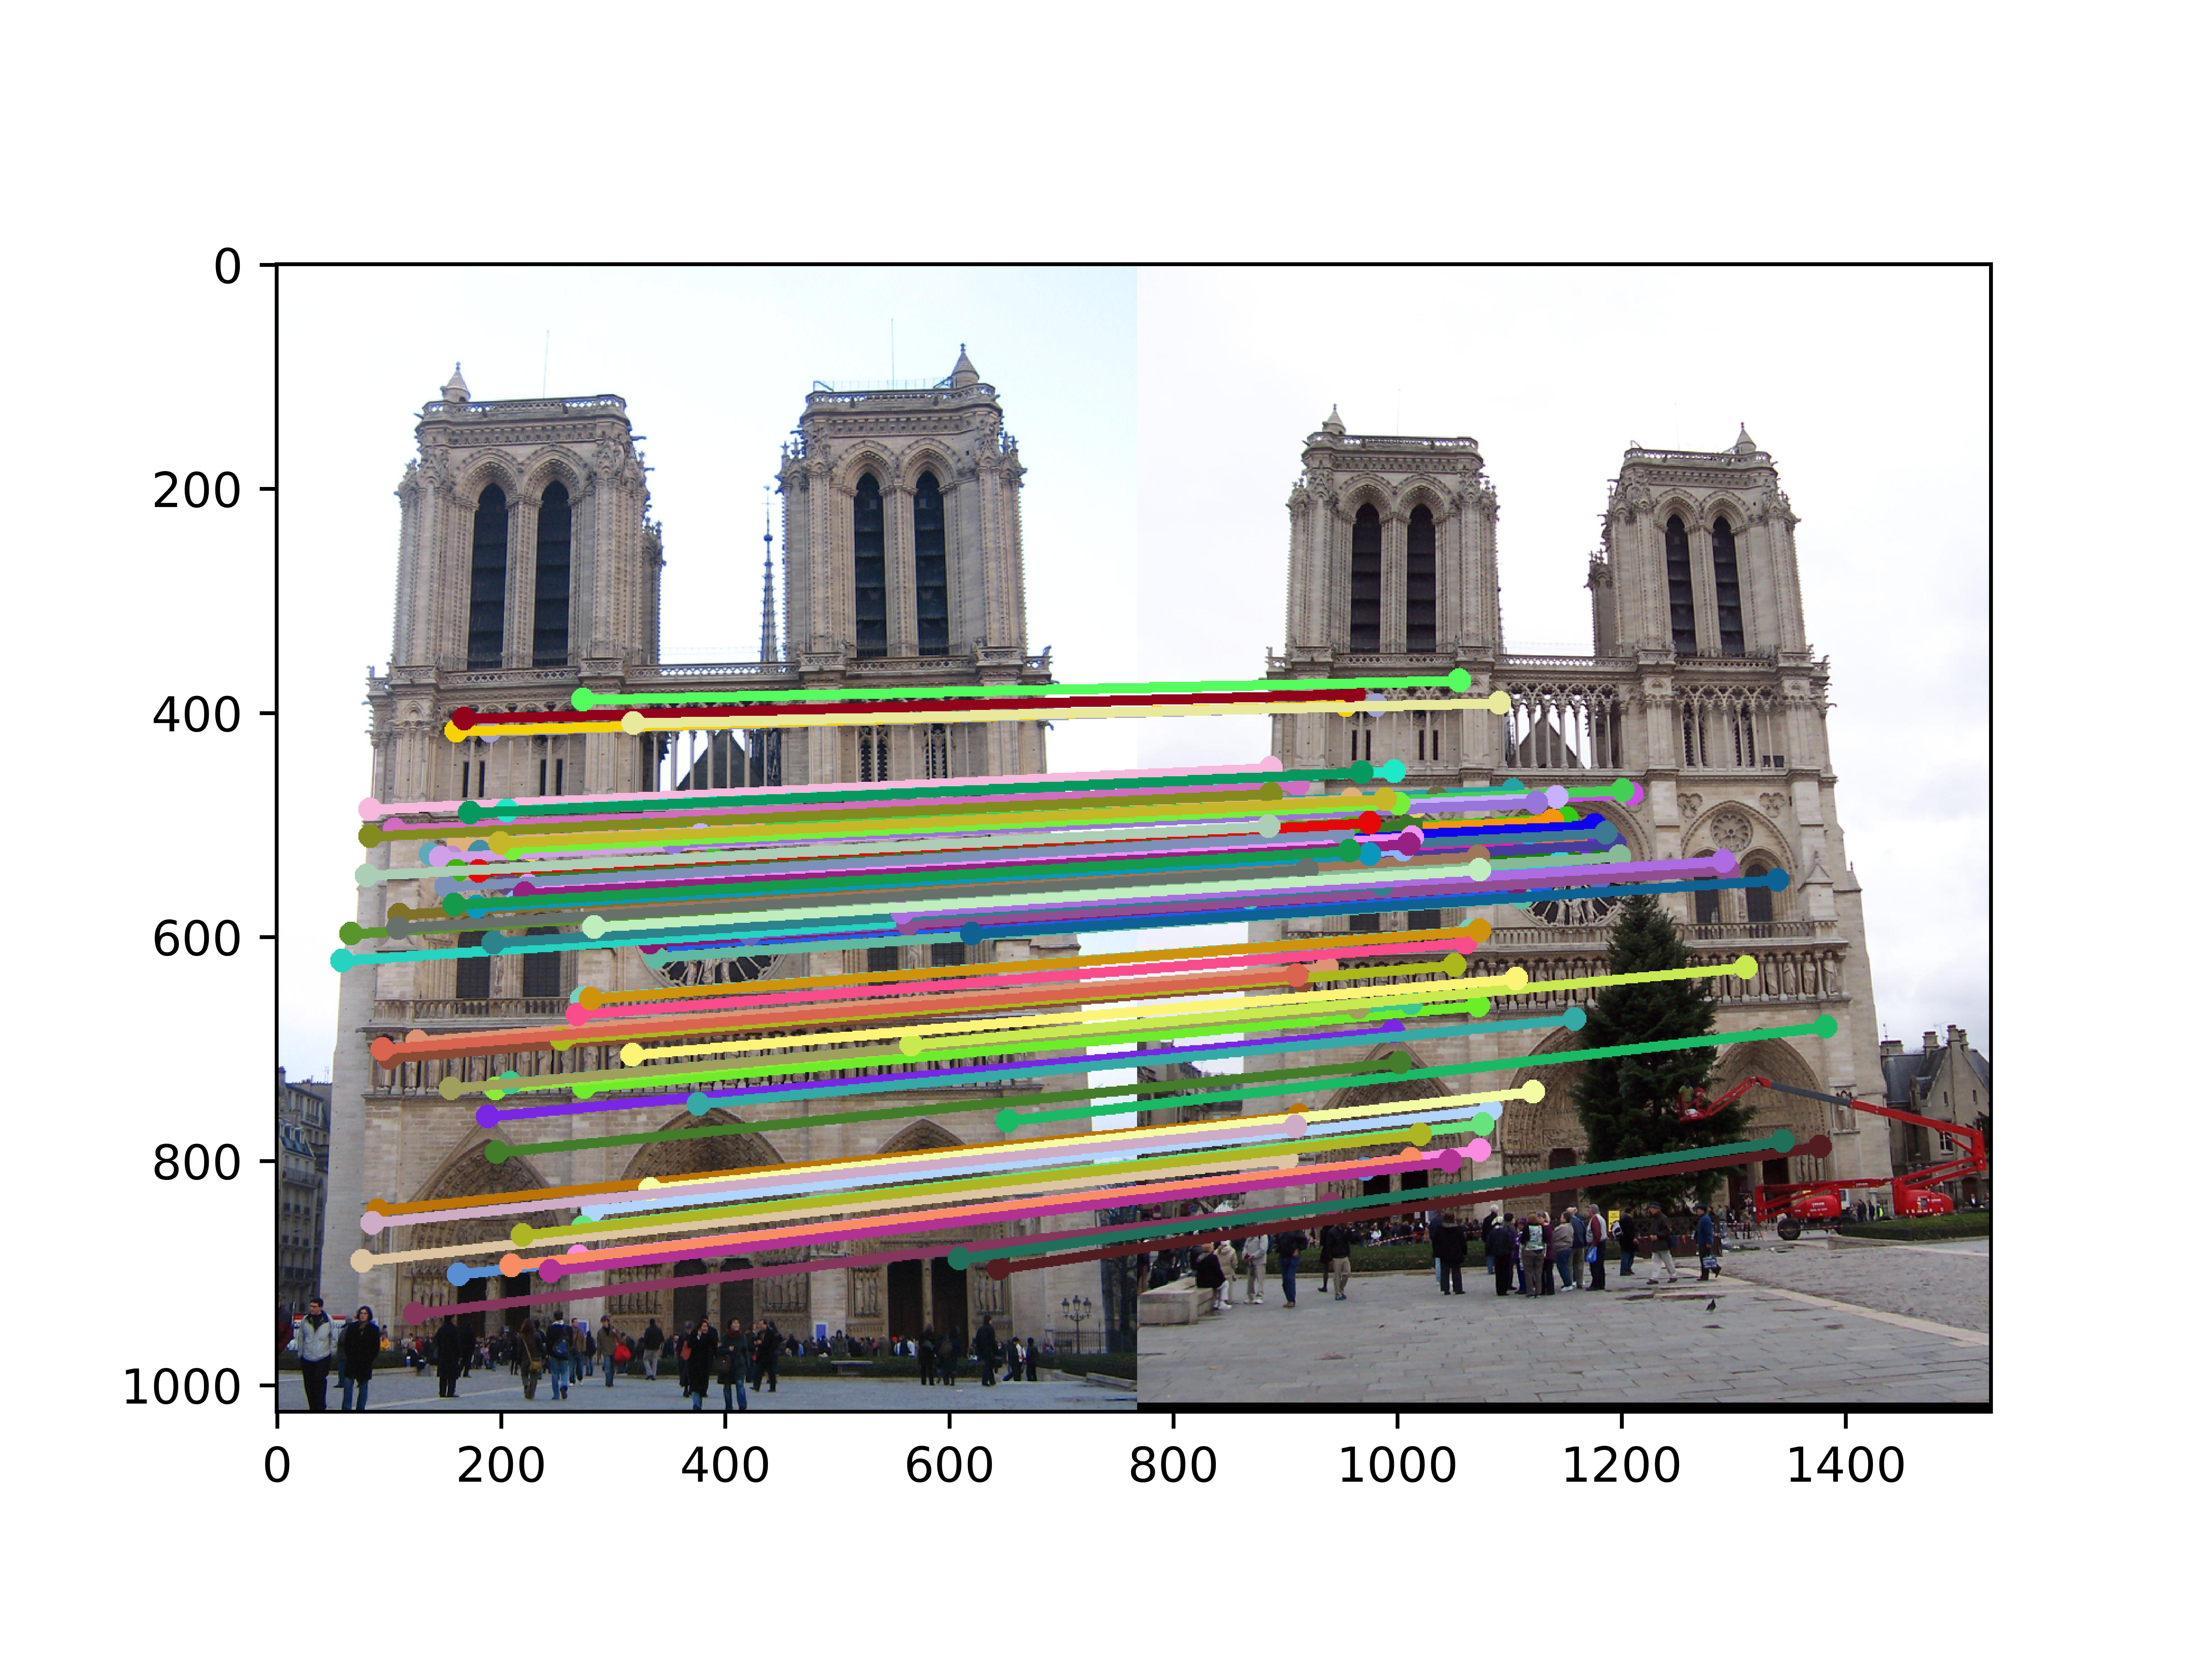
\includegraphics[width=0.5\textwidth]{images/results/vis_lines.jpg}
    }
    \subfloat [特征点匹配验证结果] {
        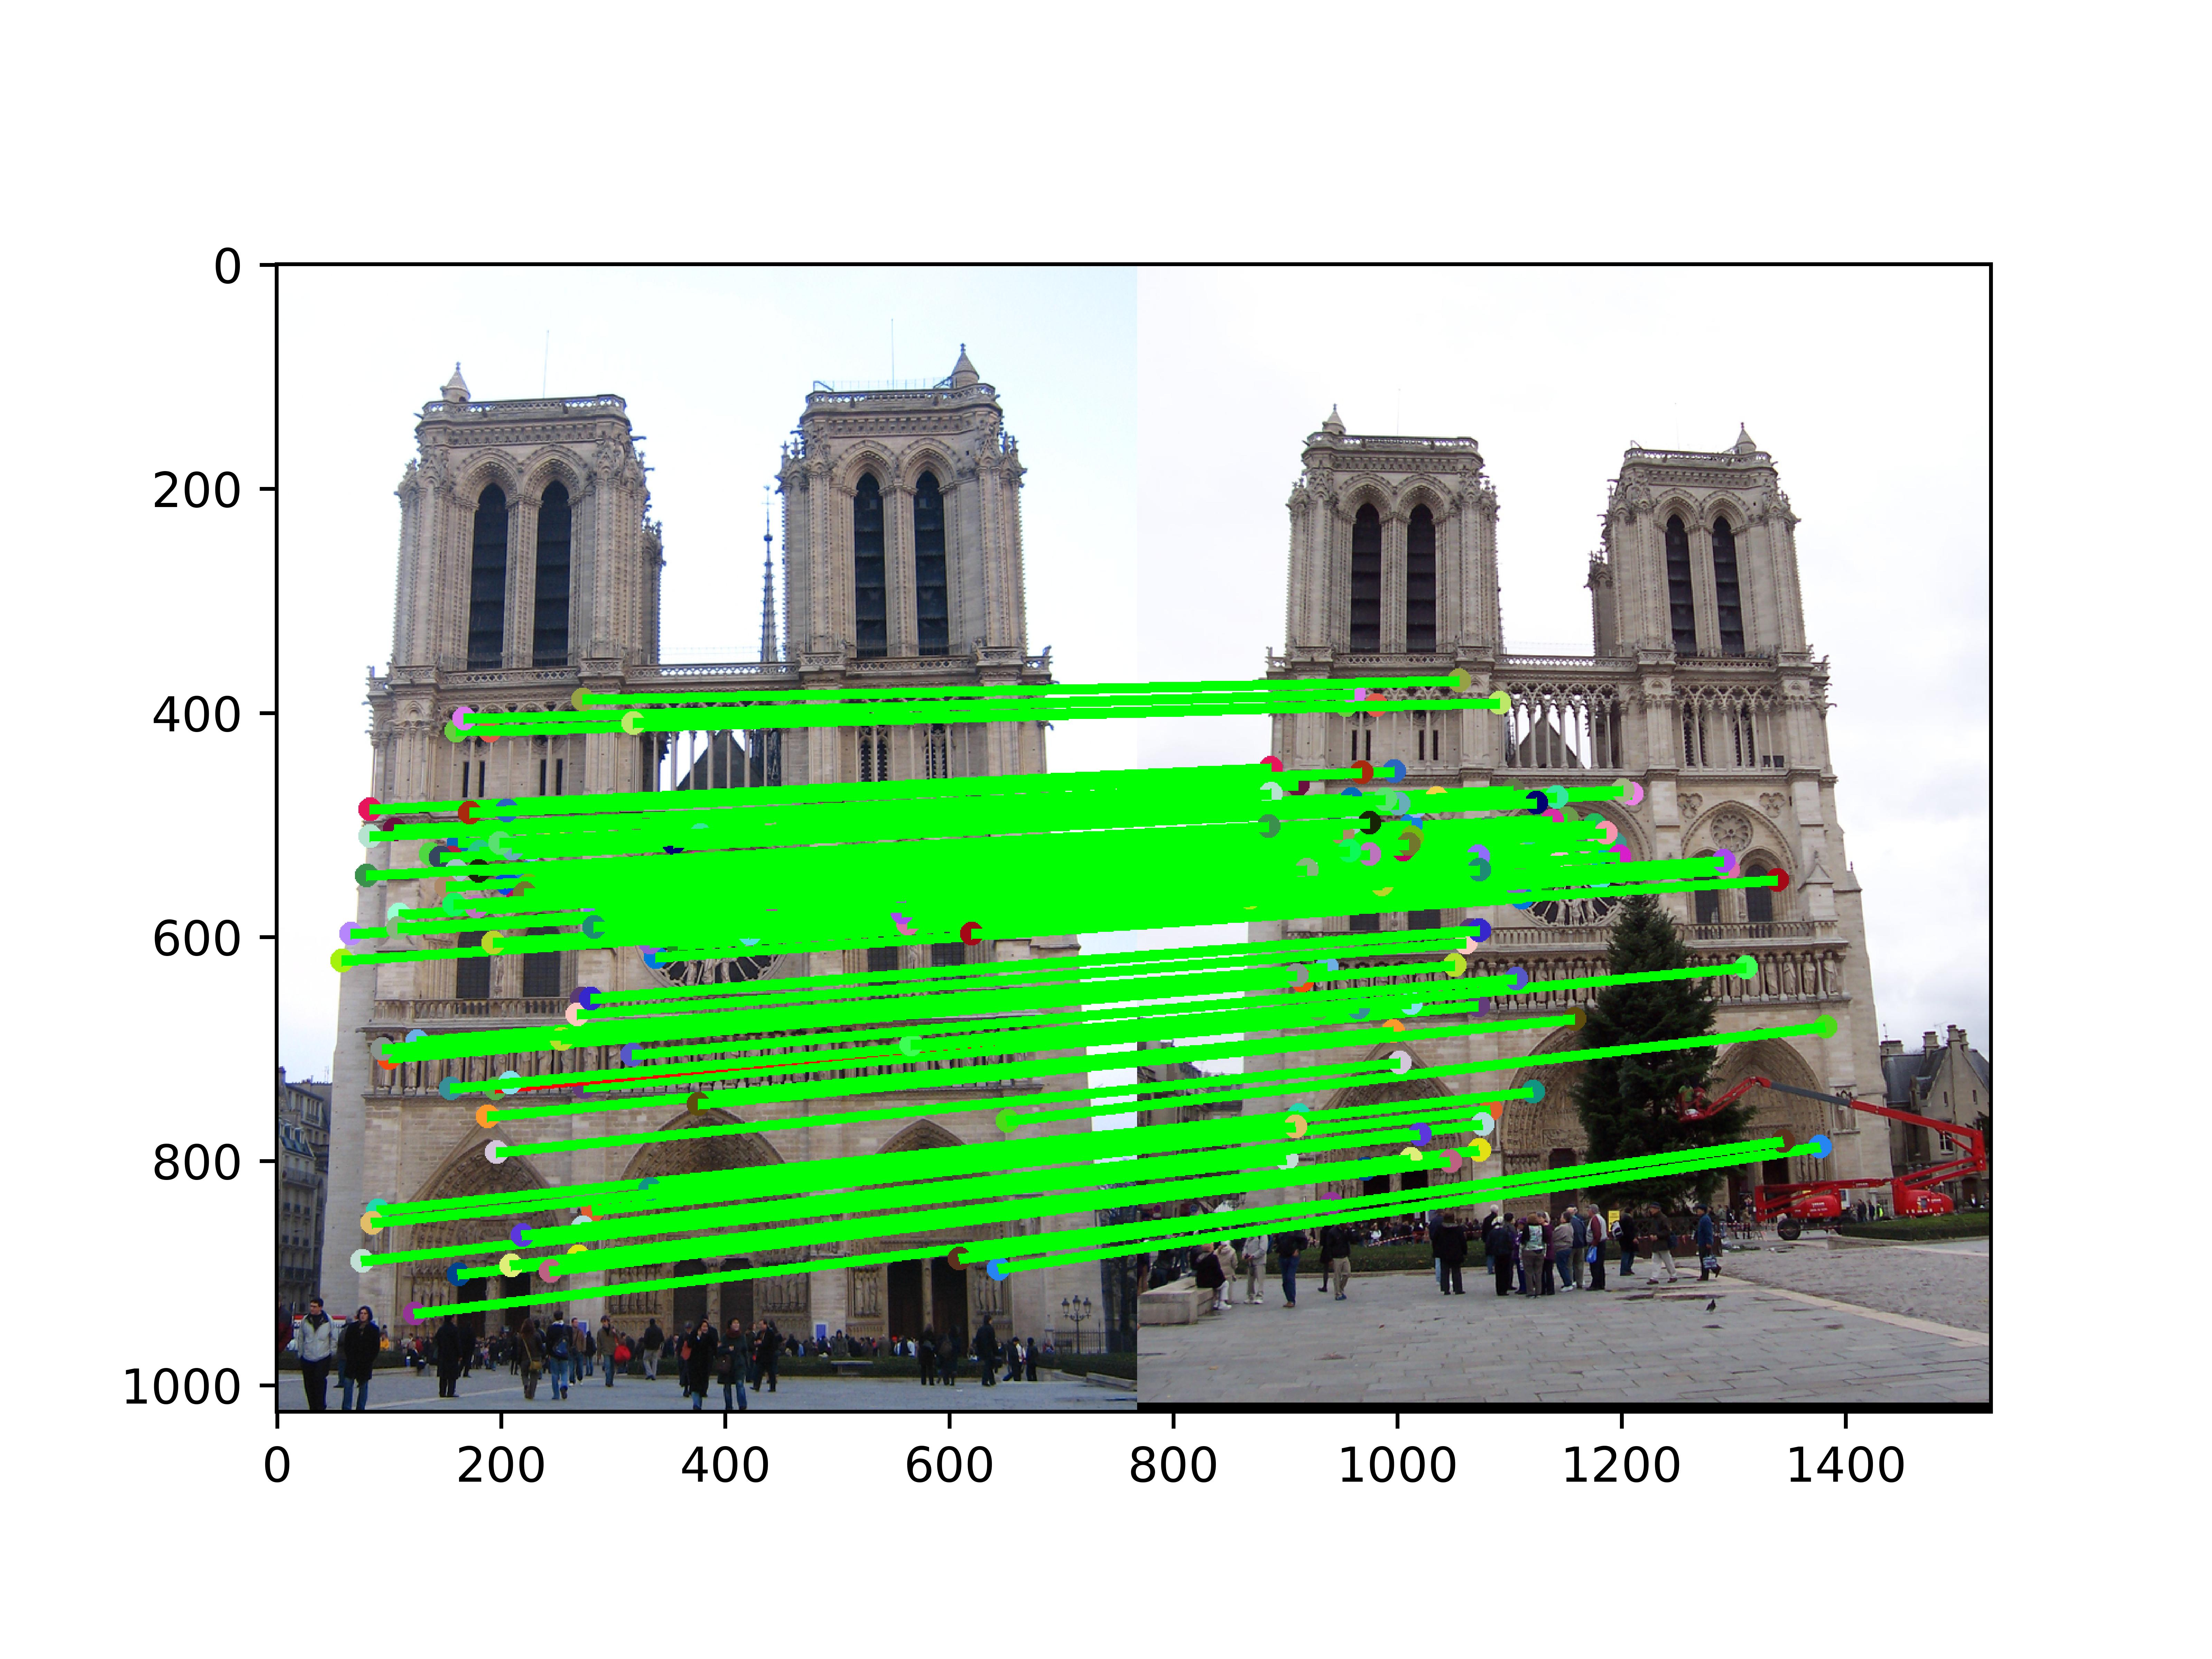
\includegraphics[width=0.5\textwidth]{images/results/eval.jpg}
    }
    \\
    \subfloat [准确率] {
        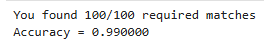
\includegraphics[width=0.5\textwidth]{images/acc.png}
    }
    \caption{实验结果}
    \label{fig:results}
\end{figure}

子图(a)展示了中间的日志信息,展示了每个过滤器排除的匹配数量,注意到每个过滤器都能够排除一部分匹配结果,可能有重复,最终的匹配结果是所有过滤器的交集。经过过滤,3099个角点最终保留171个匹配。

子图(b)展示了特征点的检测结果,其中每个特征点都用一个圆圈表示。子图(c)展示了特征点的匹配结果,其中两两特征点之间用一条线连接。子图(d)展示了特征点匹配的验证结果,其中正确的匹配用绿色线连接,错误的匹配用红色线连接。子图(e)展示了准确率信息,可以看到准确率达到了99\%。

\subsection{消融实验}

为了分析每个过滤器的作用,我们进行了消融实验,分别对每个过滤器调整参数,观察最终的匹配结果。

% 6张子图网格排列,images/abl/accuracy_vs_distance_mode.png, images/abl/accuracy_vs_distance_alpha.png, images/abl/accuracy_vs_cosine_alpha.png, images/abl/accuracy_vs_ratio_thresh.png, images/abl/accuracy_vs_spatial_cosine_thresh.png, images/abl/accuracy_vs_spatial_dist_thresh.png
% A B
% C D
% E F
% use \subfloat
\begin{figure}[H]
    \centering
    \subfloat [距离过滤器模式] {
        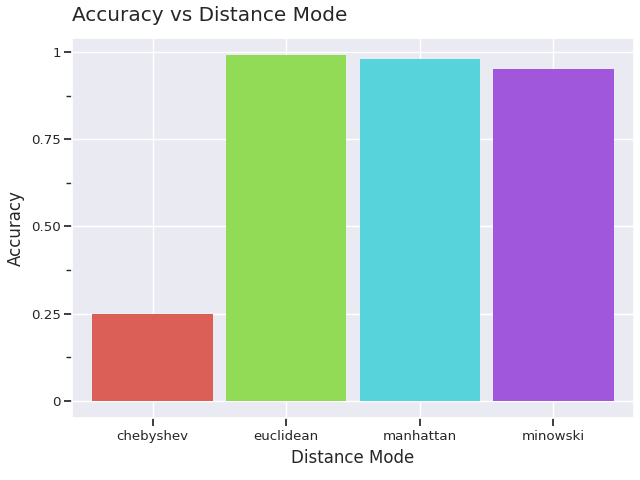
\includegraphics[width=0.33\textwidth]{images/abl/accuracy_vs_distance_mode.png}
    }
    \subfloat [距离过滤器参数$\alpha$] {
        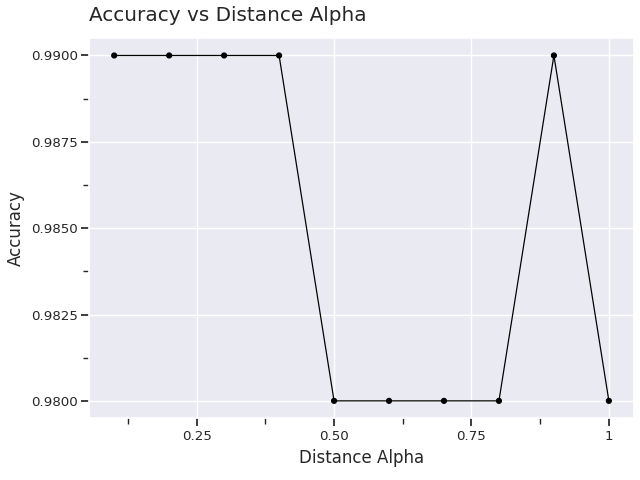
\includegraphics[width=0.33\textwidth]{images/abl/accuracy_vs_distance_alpha.png}
    }
    \subfloat [余弦相似度过滤器参数$\alpha$] {
        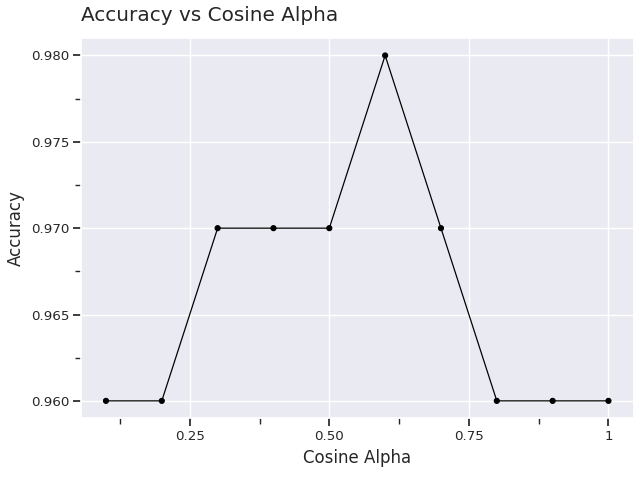
\includegraphics[width=0.33\textwidth]{images/abl/accuracy_vs_cosine_alpha.png}
    }
    \\
    \subfloat [距离比例过滤器阈值] {
        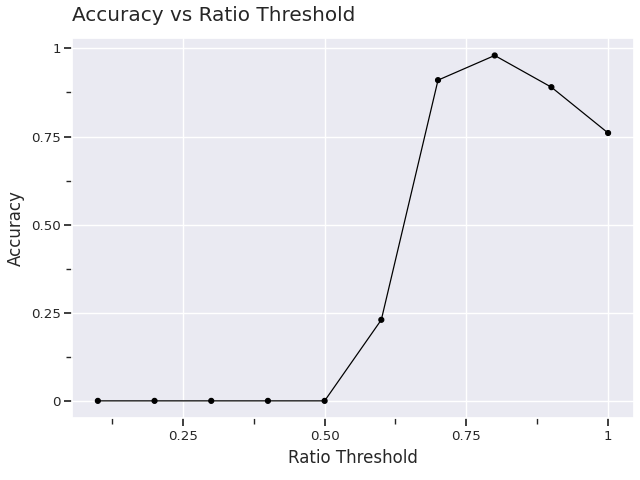
\includegraphics[width=0.33\textwidth]{images/abl/accuracy_vs_ratio_thresh.png}
    }
    \subfloat [空间过滤器参数$\tau$] {
        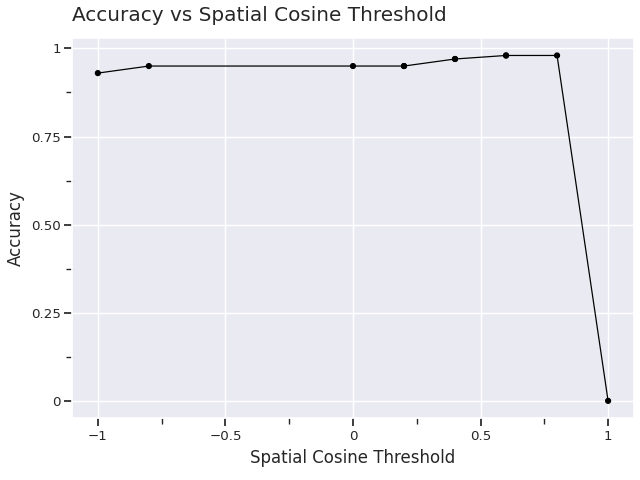
\includegraphics[width=0.33\textwidth]{images/abl/accuracy_vs_spatial_cosine_thresh.png}
    }
    \subfloat [空间过滤器参数$\gamma$] {
        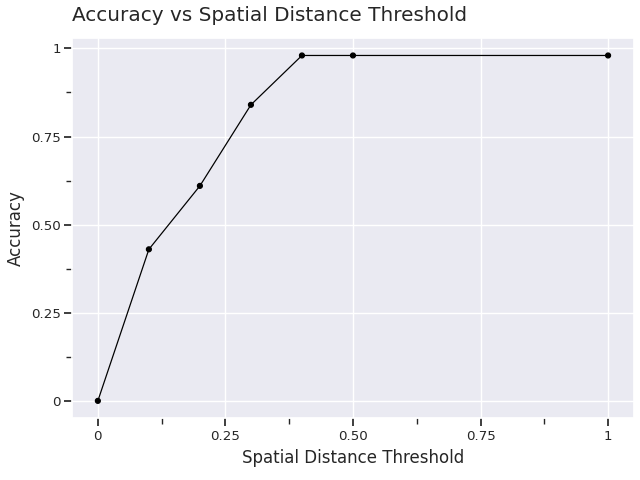
\includegraphics[width=0.33\textwidth]{images/abl/accuracy_vs_spatial_dist_thresh.png}
    }
    \caption{消融实验}
    \label{fig:abl}
\end{figure}

图\ref{fig:abl}展示了消融实验的结果,包括距离过滤器模式、距离过滤器参数$\alpha$、余弦相似度过滤器参数$\alpha$、距离比例过滤器阈值、空间过滤器参数$\tau$和空间过滤器参数$\gamma$。

子图(a)展示了不同距离度量方式的效果,可以看出欧氏距离的效果最好。

子图(b)(c)展示了距离和余弦相似度过滤器不同参数的效果,可以看出距离过滤器参数$\alpha<0.4$,余弦相似度过滤器参数$\alpha=0.6$时的效果最好。

子图(d)展示了距离比例过滤器不同阈值的效果,可以看出阈值为0.8时效果最好。

子图(e)(f)展示了空间过滤器不同参数的效果,可以看出参数$\tau=0.6$,$\gamma>0.4$时效果最好。

为了进一步展示交叉验证过滤器和空间过滤器的效果,\ref{fig:wo}中展示了去除过滤器之后的匹配结果。

% 2张子图左右排列,images/abl/wo_cross.jpg, images/abl/wo_spatial.jpg
% A B
% use \subfloat
\begin{figure}[H]
    \centering
    \subfloat [去除交叉验证过滤器] {
        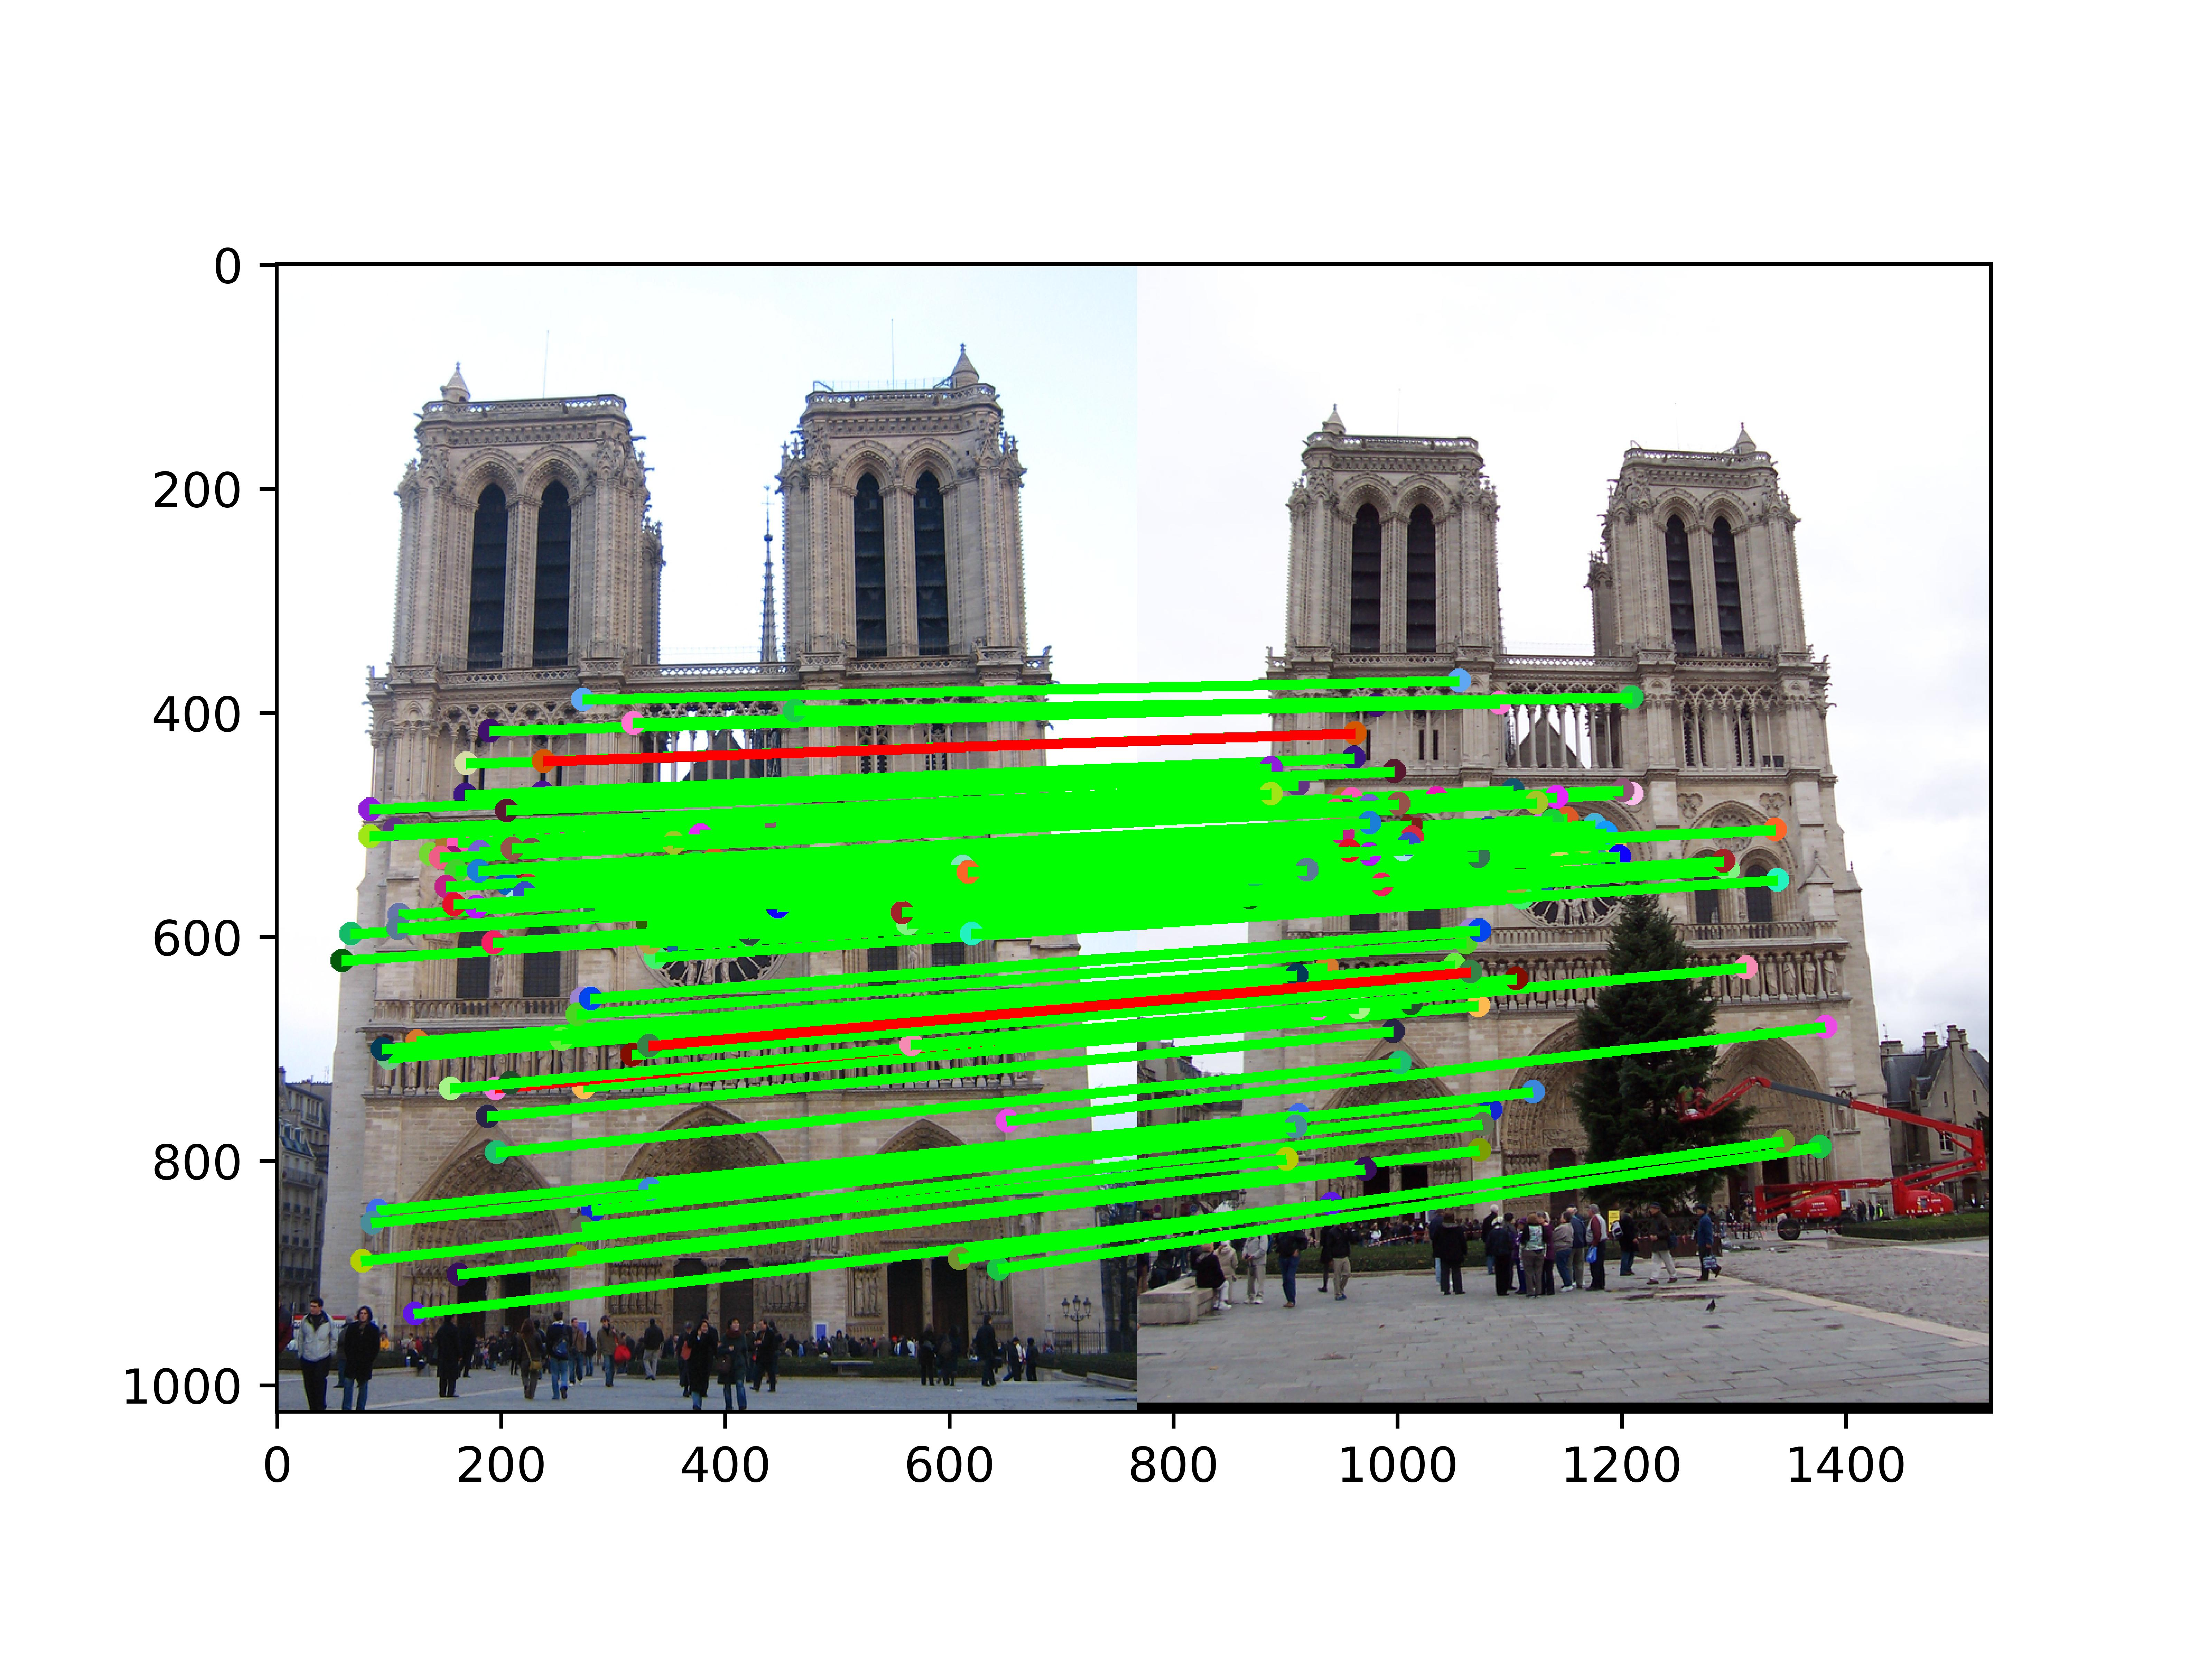
\includegraphics[width=0.5\textwidth]{images/abl/wo_cross.jpg}
    }
    \subfloat [去除空间过滤器] {
        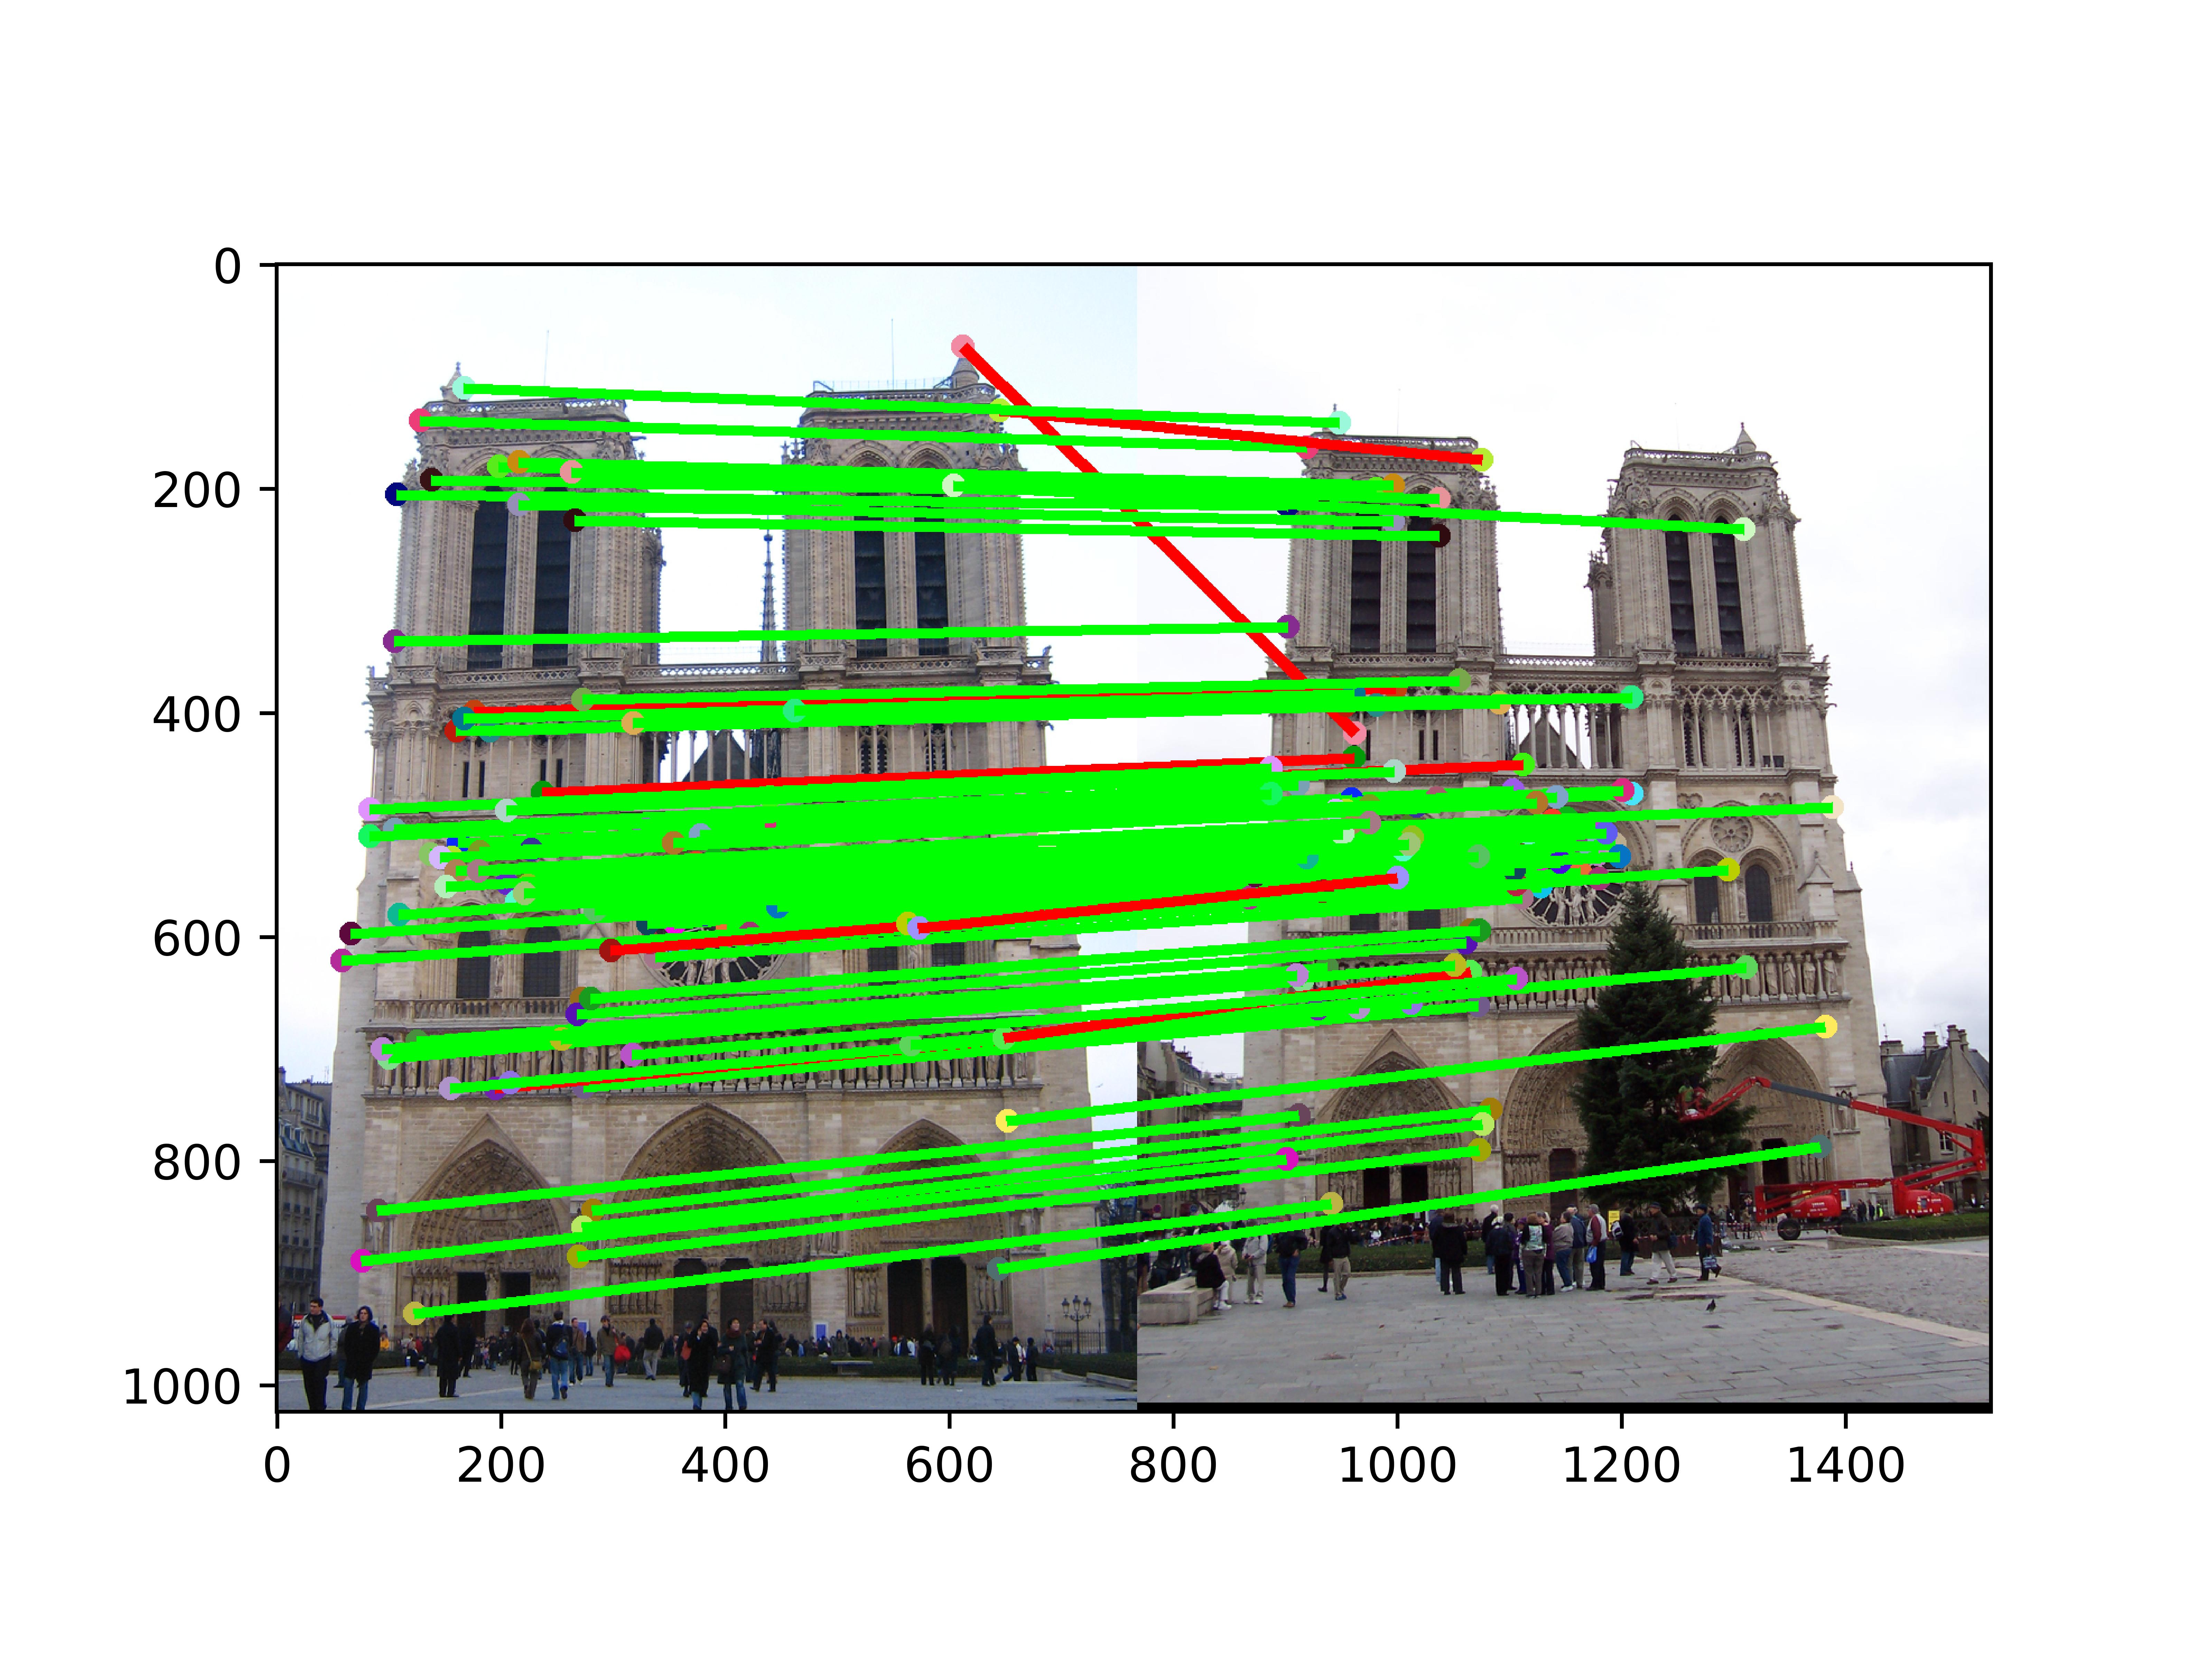
\includegraphics[width=0.5\textwidth]{images/abl/wo_spatial.jpg}
    }
    \caption{去除过滤器的匹配结果}
    \label{fig:wo}
\end{figure}

如图\ref{fig:wo}所示,去除交叉验证过滤器和空间过滤器之后,匹配结果明显变差。其中子图(a)展示了去除交叉验证过滤器之后的匹配结果,去除之后,结果中出现了一对多的匹配。子图(b)展示了去除空间过滤器之后的匹配结果,去除之后,结果中出现了一些方向和距离与总体趋势不一致的匹配,进一步说明了交叉验证和空间过滤器的重要性。

\subsection{实验分析}

本次实验实现了一个基于特征点的图像匹配算法,该算法包括特征点的检测与匹配,以及匹配结果的验证。通过实验验证了该算法的有效性,通过距离度量函数和过滤器的设计,实现了高达99\%准确率。

图像特征点的检测是图像处理中的一个重要问题,主要的方法有Harris角点检测算法、SIFT算法、SURF算法等。不同方法具有不同的特点,其中:

\begin{itemize}
    \item Harris角点检测算法是一种基于图像梯度的角点检测算法,通过计算图像的梯度,找到梯度变化最大的点作为角点。该算法简单易实现,且对图像的平移、旋转具有不变性,但对尺度变化不具有不变性。
    \item SIFT算法是一种基于高斯差分金字塔的特征点检测算法,通过高斯差分金字塔找到图像的极值点作为特征点。该算法通过高斯差分金字塔对不同尺度的图像进行分析,因此在一定程度上缓解了特征点随尺度变化的问题。
\end{itemize}

两种算法的详细介绍请参见实验原理部分,这里对两种算法的不变性进行分析。一个像素点$(x, y)$的梯度是通过与相邻像素点的值相减得到的,可以表示为公式\ref{eq:grad}:

\begin{equation}
    \label{eq:grad}
    I(x, y) = (x, y) - (x - 1, y - 1).
\end{equation}

平移操作可以表示为公式$(x', y')=(x + t_x, y + t_y)$,其中$(x, y)$是原始图像的坐标,$(x', y')$是平移后的图像的坐标,$(t_x, t_y)$是平移的距离。对于平移操作,平移前后的梯度$I(x, y) = I(x', y')$,因此Harris角点检测算法对平移具有不变性。

旋转操作可以表示为公式$(x', y')=(x \cos \theta - y \sin \theta, x \sin \theta + y \cos \theta)$,其中$(x, y)$是原始图像的坐标,$(x', y')$是旋转后的图像的坐标,$\theta$是旋转的角度。对于旋转操作,旋转前后的同一像素点的梯度的两个主方向具有相同的特征值,因此Harris角点检测算法对旋转具有不变性。

缩放操作可以表示为公式$(x', y')=BLI(s_x x, s_y y)$,其中$(x, y)$是原始图像的坐标,$(x', y')$是缩放后的图像的坐标,$(s_x, s_y)$是缩放的比例,$BLI$是双线性插值。对于缩放操作,缩放前后的像素点与相邻像素点的值被改变,因此Harris角点检测算法对缩放不具有不变性。

SIFT算法则是另一种思路。SIFT算法对图像的不同尺度计算高斯金字塔,之后进行差分。高斯模糊操作通过一个高斯卷积核对图像进行卷积来实现,卷积操作可以表示为公式\ref{eq:convlution}:

\begin{equation}
    \label{eq:convlution}
    I(x, y) = \sum_{i=-\infty}^{\infty} \sum_{j=-\infty}^{\infty} K(i, j) I(x - i, y - j),
\end{equation}

其中$I(x, y)$是卷积后的图像,$K(i, j)$是卷积核,$I(x - i, y - j)$是原始图像。对于平移操作,相同的像素点与周围像素点的值相同,卷积得到的结果相同。因此SIFT算法对平移具有不变性。对于旋转操作,高斯卷积核的等高线呈圆形,旋转不会改变卷积核中对应元素的值,因此SIFT算法对旋转具有不变性。

对于缩放操作,像素周围的值被改变,卷积得到的结果也会改变,因此SIFT算法对缩放不具有不变性。然而,SIFT算法通过高斯金字塔对不同尺度的图像进行分析,因此在一定程度上缓解了特征点随尺度变化的问题。

综上所述,SIFT算法具备更好的性能,因此本实验选择了SIFT算法作为特征点检测算法。在特征点匹配方面,本实验首先通过暴力匹配算法找到匹配点对,之后通过距离过滤器、余弦相似度过滤器、距离比例过滤器和空间过滤器对匹配点对进行过滤,最终得到了高准确率的匹配结果。对于这些过滤器的详细介绍和分析,请参见实验步骤和消融实验部分。